\onehalfspacing

\section{Software}

\noindent The initial part of the project involved becoming familiar with the various technologies that are being used to analyse the data at NO$\nu$A. The data and software used to analyse the data are stored on the High Energy Physics group’s Linux cluster of machines, running both Scientific Linux, meaning that it was essential understand the Linux command line in order to navigate the file system and software packages, as well as run and debug scripts. \medskip

\noindent NO$\nu$ASoft is a software package, developed by Fermilab, that builds on the ROOT data analysis software \cite{Brun}, developed by CERN. CAFAna is the framework that NO$\nu$ASoft uses to run functions and produce plots by specifying cuts on the data. The  analysis framework is written in C++, a language I had no prior experience of, so a proportion of the time was spent trying to interpret pre-existing C++ scripts in NO$\nu$ASoft, as well as the doxygen documentation. \medskip



\section{Training data}

\noindent The MC data is stored as ROOT files, as well as HDF5 files that contain the training data. The image data comes in the form of an array and the interaction targets in the form of a ‘pdg’ (particle data group) value. The event labels are stored as part of ‘mc’ branch of the HDF5 file, while the input images are stored in a ‘training’ branch. \medskip

\noindent The data stored in these HDF5 files has already undergone preselection cuts- this was indicated by the fact that the number of subevents stored in the ‘mc’ branch is larger than that of the ‘training’ branch. Because of this, the events could not simply be matched up based on their index value, but on the following values: ‘run’, ‘subrun’, ‘evt’ (event), ‘subevt’ (sub event) and ‘cycle’ to indicate which subevent is being referenced. \medskip

\noindent After reshaping the image maps from a 1D array to two 100 x 80 pixel images representing the z-x and z-y planes of the detector (see Figure 7 for plots of an event in the two detector planes), the images were written to a 4D tensor with dimensions:
{\begin{itemize}
 \vspace*{-3mm}
\item event index (determined by the order that the images were added),
 \vspace*{-3mm}
\item plane (z-x or z-y),
 \vspace*{-3mm}
\item z value,
 \vspace*{-3mm}
\item x or y value.
 \vspace*{-3mm}
  \end{itemize}}
    
\begin{figure}[t!]
 \centering
 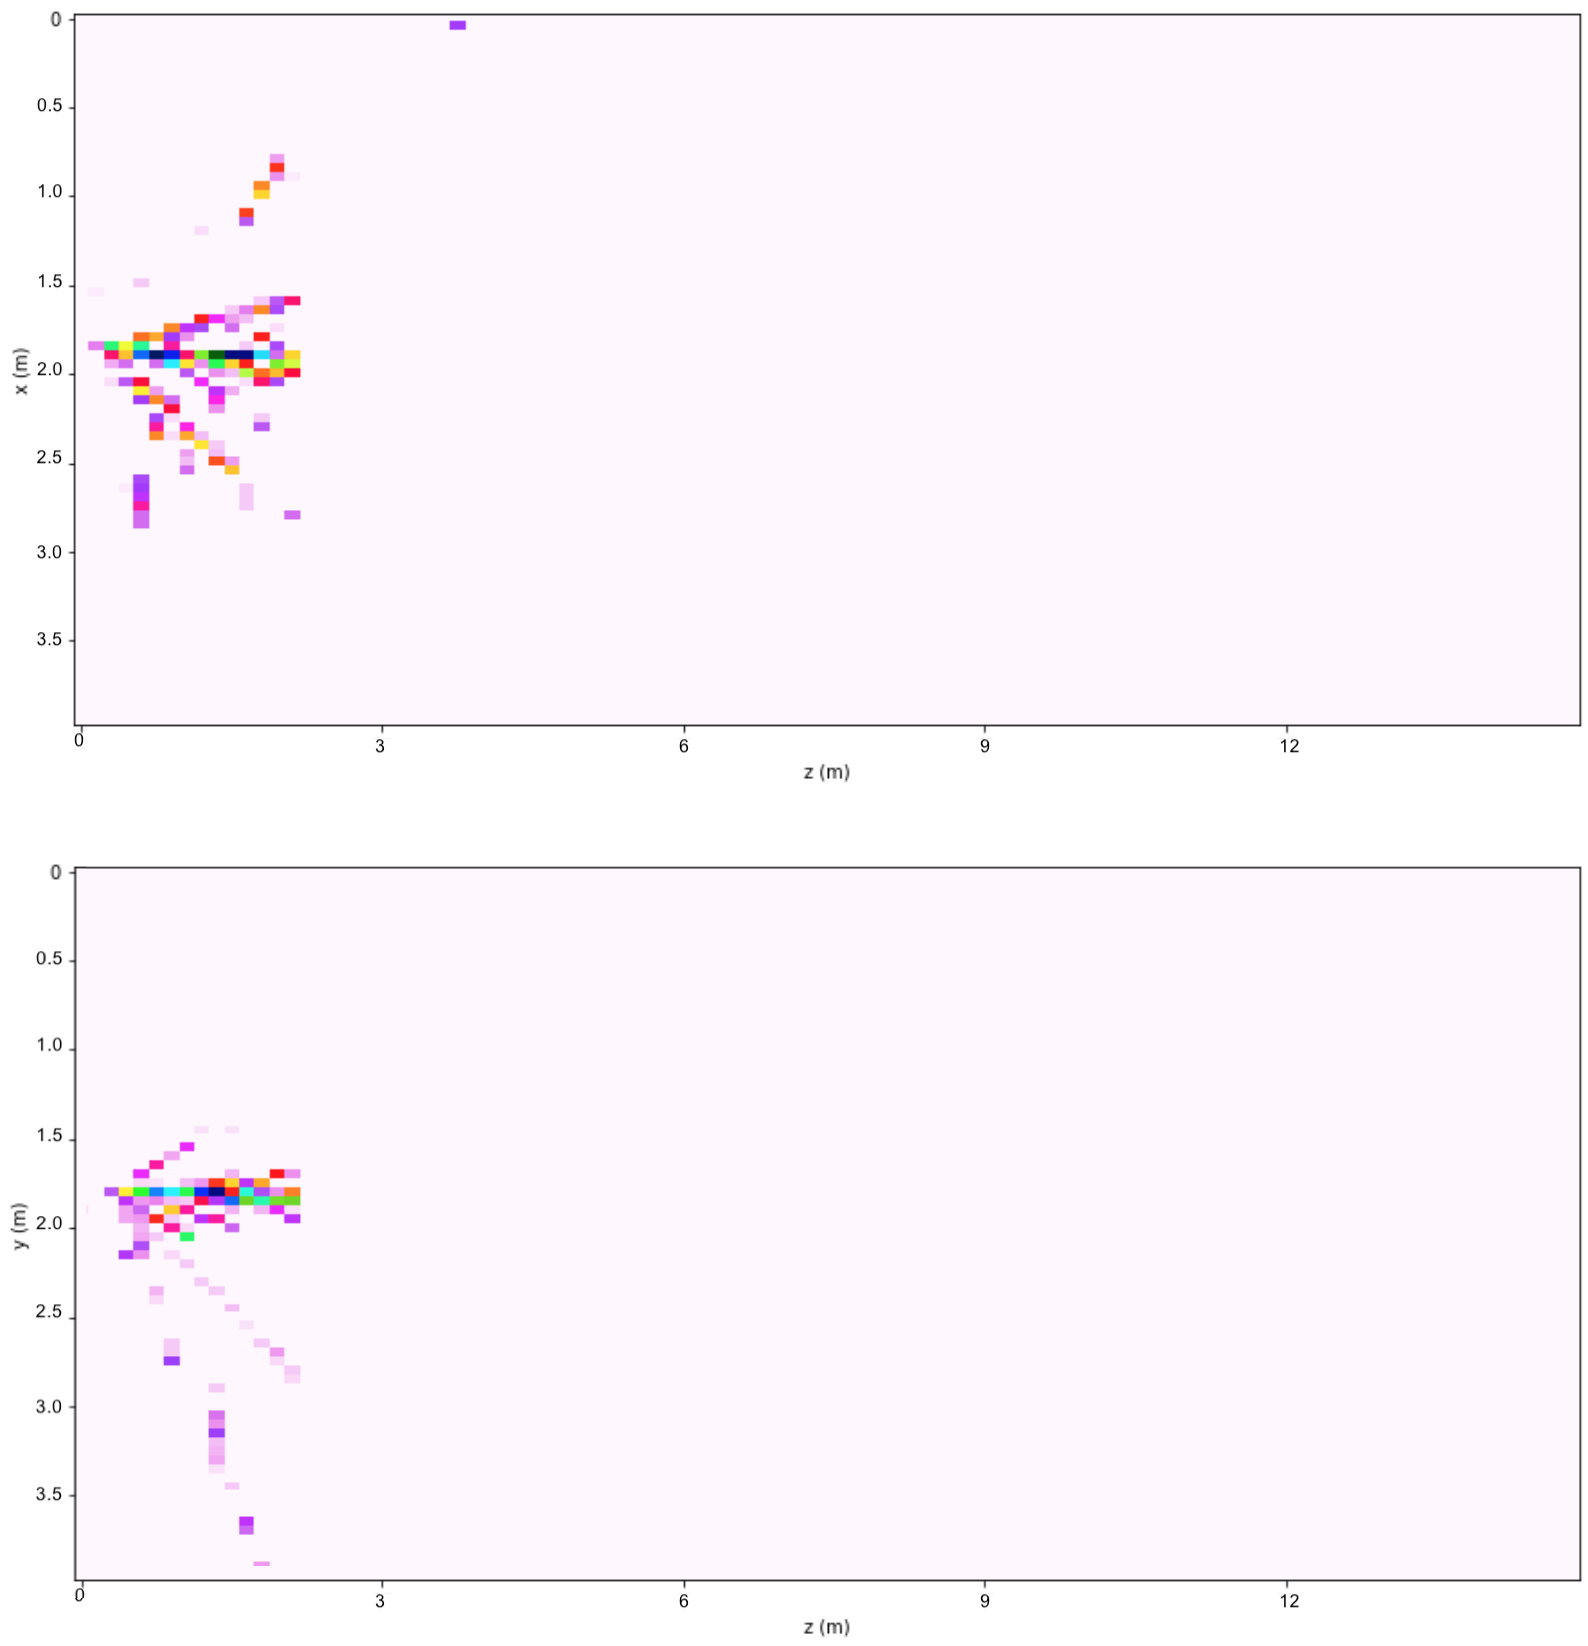
\includegraphics[width=120mm]{Images/xyzplots.png}
 
 \textbf{Figure 7.} \textit{Plot showing an event from the two planes of the detector (z-x and z-y) .}
\end{figure}

\noindent The HDF5 files also store data about each event, and this was used to apply the basic quality and preselection cuts. The cuts were outlined in the NO$\nu$A doxygen with the $\nu_\mu$ cuts as to remove any events that could be considered background events. These could be, for example atmospheric neutrinos, as well as neutrinos produced on earth, or from another process, and would be removed by the Cosmic Rejection cuts and the preselection cuts, as well as basic quality cuts.\medskip

\noindent Much like the the code already for the NO$\nu$A project and NO$\nu$Asoft, these are written in C++ and use the branch like structure of the ROOT files. A package has been developed for Python, called Pandana, however, I am unfamiliar with the syntax associated with the package and the documentation seems to focus on network analysis, so I deemed it a simpler option to simply implement the cuts using if statements with a loop over all the events. \medskip

\noindent While this meant that the computational process is much slower, I didn't see that as a problem as the cuts need only be applied once, for each generator, and the events that pass can be stored and then used as model inputs from then onward. In order to verify that the cuts that I had made were correct, a function had been written in NO$\nu$ASoft, ‘MakeEventListFile’, that listed the events that pass a specific cut, in order to be able to cross reference with the results I obtained.\medskip

\noindent It may be useful to learn and then implement the Pandana approach if more training data needs to be used in the future, or if the network was to be trained dynamically in the future.\medskip

\noindent While Keras does have a C++ API, as well as the option to export a model from Python, as Python is the language I am more comfortable with I decided that it was worthwhile interpreting the cuts and implementing them in Python rather than using the pre-existing C++ functions.\medskip

\section{Models}

\noindent The data that passed the preselection cuts, now in the form of image maps and labels indicating the interaction type, were now able to be passed to a model for training. Initially this was done on a smaller scale, using just 10 of the available 1150 files in order to ensure that all components were working properly. The interaction labels are one hot encoded into three classes: neutral current (NC), charged current  (CC) $\nu_e$  (and  ${\overline{\nu}_e}$) , CC $\nu_\mu$  (and  ${\overline{\nu}_\mu}$) as the classifier makes predictions for if an event belongs to each class.\medskip

\noindent Initially I produced a small network containing 6 sequential blocks containing convolution, max pooling and drop out layers in Keras. I did this to understand whether there were any errors in the formatting of the data as I was familiar with what was required for my rudimentary model. This worked with no hiccups, although the classifier was not particularly accurate. \medskip

\noindent The next stage was to run the small dataset using the MobileNet \cite{Sandler} architecture, developed by Google.  MobileNet is designed for implementation on mobile devices with a reduced computing power and thus reduced the training time significantly. As the computational facilities at the HEP Linux cluster I was using for the project do not have GPU cores to train the models, this more memory and processor efficient network made training more efficient that even my simple sequential network, despite being a more complex and having a much larger number of trainable parameters.\medskip

\noindent Literature stated that MobileNet does experience a reduction in classification performance \cite{Brun}, however the increase in performance time is significant and more valuable to a project with a limited timeframe, which is looking to see if new methods can be implemented, as opposed to producing a final production model.\medskip

\noindent The MobileNet architecture, officially known as MobileNetV2, uses 'depthwise separable convolutions', 'linear bottlenecks' and 'inverted residuals' to improve the training time and memory efficiency. \cite{Sandler}. MobileNet applies 3 x 3 depthwise separable convolutions that replace conventional convolutions, by first applying a single convolutional filter before a 1x1 convolution builds new feature maps through linear combinations of the inputs. Linear bottlenecks project, or embed, the feature maps to a lower-dimensional spaces, and it is this projection that leads to the loss in information, but reduced training time. Rather than use a non-linear activation function such as ReLU, a linear one is used instead to prevent a loss of information during the transform. The inverted residuals act as feature map expansions from the low-dimensional space.\medskip

\noindent In this project the MobileNet architecture was altered to take in two images per event, for the two planes of the detector, and process these in parallel before concatenated them together before rest of the network processed the inputs.\medskip

\noindent The network produces probabilities for each category indicating the confidence level that the network has in belonging to each label class. By taking the category that the model is most confident of we can compare this to the MC truth data we obtain the accuracy values, and the loss values that the loss values that the training process uses to indicate the success of the training. \medskip

\section{Generator Method}

\noindent While it was possible to write the required data to an array when working with a relatively small dataset, this was not possible when using all of the available files in the directory- 1150 GENIE HDF5 files, each with approximately 8370 events, totalling 9625500 events in total.
As a result I decided to produce a data frame for the events that passed the cuts, storing the following data about the event, but not the image map itself. The columns of the dataframe were as follows:
{\begin{itemize}
 \vspace*{-3mm}
\item ‘run’ ,
 \vspace*{-3mm}
\item ‘subrun’,
 \vspace*{-3mm}
\item ‘evt’ (event),
 \vspace*{-3mm}
\item ‘subevt’ (sub event),
 \vspace*{-3mm}
 \item ‘cycle’,
 \vspace*{-3mm}
\item ‘train\_index’:  location index within the ‘training branch’ of the image,
 \vspace*{-3mm}
\item ‘label’ : pdg interaction value,
 \vspace*{-3mm}
\item ‘file’: path to the relevant HDF5 file. 
  \end{itemize}}

\noindent The data frames were then concatenated to produce three: one for training containing 335,456 sub events, one for training validation containing 67,092 sub events, and one for testing the model containing 93,248 sub events.\medskip

\noindent As the data was not stored locally, the data could not be loaded into the model all at once. Keras allows for a generator to load the data to the model in various batch sizes. This sources the image data from the relevant HDF5 file using the location stored in the ‘file’ column of the data frame and the 'train\_index' value from that row to identify the array in question. This is then reshaped the same way as before and written to a 4D tensor identical to the one for the entire dataset, with the only difference being the event index dimension is the size of the batch size that is specified, rather than the entire dataset. The default batch size is 32, as is the case with the results produced by NO$\nu$A\cite{Aurisano}. The target values are again one-hot encoded based on the ‘label’ value for the row.\medskip

\noindent The GiBUU events are similar to the genie events in the way that the data is stored in the HDF5 files, so an identical approach could be used to preselect data and store the corresponding data regarding the events in a dataframe, that also contained the location of the training images, as was with the GENIE events. The GiBUU events have an additional property, being that each event is given a weight value. These weight values were contained in the HDF5 files, however they were incorrect- with values ranging from the order of 10\textsuperscript{-3} to 10\textsuperscript{4}. A NO$\nu$ASoft function had been written to correct this, but as I was not using the ROOT files, but the HDF5 files I could not directly apply the function to the values in the HDF5 files. As well as this the function relied on a large number of C++ dependency files that made it an unreasonable task to try and replicate the function in Python, as had been done with the preselection cuts.\medskip

\noindent Once again the ‘MakeEventListFile' function could be used to create a text file with the associated weight value for each event. Then a mapping function could be used to add the weight value to the correspoding event.\medskip

\noindent In the training process the weight was used to provide a the weighing that each particular event should have on the overall statistics of the dataset. In our case that indicated the importance of the event to the training process. I was unable to find a method in Keras that allowed for a weighted training procedure, that being one where the magnitudes of the gradients calculated for the gradient descent backpropagation process were scaled in accordance with the GiBUU weights. This gradient scaling was used when training the DANN as will be discussed later, however every event was scaled by a constant value in that case, rather than changing for every event here. The tensor batch preprossessing in the MobileNet architecture applies a 'Subnet' process to the batch that meant that I could not ensure that the associated weight would correspond correctly when calculating the gradients for each event without extensive testing that I did not think could be completed within the timeframe of the project.\medskip

\noindent Alternatively, the weight was used as a value that indicated the likelihood that the event would be included in the training procedure. A random number was generated between 1 and 10, which was the range in which almost all of the weights values were contained, with the exception of a few that were greater in value. If the weight value of an event that had passed the preselection cuts was greater than the random generated value the event data was written to the dataframe. If it was lower it was passed and the next event was evaluated in the same way.As the GENIE events did not contain this weight value, all the GENIE events that passed the preselection cuts were written to the train, validate and test dataframes.\medskip

\noindent This process did mean that a large proportion of the GiBUU events were not used in the training process, however this was not as large of a problem, as the number of GiBUU events given far exceeded the number of GENIE events available, and as will be discussed in the imbalanced dataset section, as we as the computational expense section, I would not have been reasonable to train the model using all of these events anyway.\medskip

\noindent Once these dataframes had been produced, a generator function could load in the data to the models for training.

\section{Hyperarameters}

\noindent A neural network is defined by a number of hyperparamters, which are parameters that are defined in order to build the model and include the number of hidden layers, the number of nodes in dense layers, the learning rate, the optimiser as some examples.\medskip

\noindent The majority of these values are predefined by the MobileNet network architecture, and thus were remained unchanged when training and testing (but were altered when the network was stripped back for debugging purposes), these include the network architecture regarding the depth and width of the network, the activation functions- which are the non-linear functions that are applied as the output of a node, the reguliser- which applied penalties to layer operations to avoid exploding, or vanishing of gradients, and the dropout values- which are the percentage of nodes that are zeroed during that training epoch to avoid overfitting. \medskip

\noindent The hyperparamters that were experimented with were the batch size of the network- which is the number of samples that are processed at one time when calculating the backpropogation gradients, the learning rate- which is a value that determines how much the weights are adjusted when learning (this can be variable), the optimiser - the algorithm that looks to reduce the loss function by finding the global minimal- as there are too many unknowns to calculate the optimal network, the problem becomes one of a  optimisation problem, and the loss function- the calculation of how the classifier performs against the truth value by looking at the residual between these. \medskip

\noindent For each hyperparameter, there were a number of options to try and determine the optimal combinations.For the optimiser the two options used were the ADAM optimiser \cite{Kingma}, and Stochastic Gradient Descent \cite{Guo}. Adam uses an adaptive learning rate and takes advantage of momentum by using moving average of the gradient instead of gradient itself like SGD with momentum. SGD replaces the actual gradient (calculated from the entire data set) by an estimate (calculated from a randomly selected subset of the data). The Adam optimiser proved more effective, and was used throughout. \medskip

\noindent For the loss function, as this is a classification task, the most sensible option was to use a categorical cross entropy, as opposed to a mean squared error used in regression, or spare categorical cross entropy, which is used when the labels are given as an integer, rather than a vector. The reason that the labels were one-hot encoded rather than input into the model as integers is because the model then does not assume anything about a larger integer label having some sort of greater value, or that class 1 is closer in nature to class 2 than class 3, for example. \medskip

\section{Data Imbalance}

\noindent By the nature of the production mechanism in which the $\nu_e$ are produced in the beam, at the near detector the number of $\nu_e$ events in comparison to the number of NC events and $\nu_\mu$ events is incredibly small (1 $\nu_e$ event for each 19 $\nu_\mu$ events).\medskip

\noindent While providing data with these proportions to the model will give the model an accurate description of the nature of events that are detected by the near detector, the model will naively weight the $\nu_\mu$  events are more important due to their abundance, and completely disregard the $\nu_e$  events, and to a lesser extent the $NC$ events. \medskip

\noindent By simply predicting every event to be that of a muon neutrino, the model would obtain an accuracy of 65\% however the classifier would be completely useless in identifying a $\nu_e$. In order to prevent this from taking place, as well training the model to develop a better understanding of the indicators that a $NC$ or $\nu_\mu$ event had taken place, a balanced data set was provided to the network.\medskip

\noindent This was completed by altering the generator function to accept events based on a number of criteria, and to reject some- that is, not passing them onto the model for training in that instance. The generator would produce a series of random values, and if each value was above a threshold value then the event would be passes onto the model. The thresholds were set for whether the event was a muon neutrino event, a charge neutral event and if the event is a GiBUU generated event using the weighting associated with that event.\medskip

\noindent By preselecting the events in such a way, much like the preselection cuts, the number of trainable events was again reduced by 93\%. Machine learning algorithms require large amounts of data to be able to determine the weights, especially deep learning models. The MobileNet model contains 394,548 trainable parameters and these methods that do not utilise all the available data significantly reduces the model's ability to set each weight and bias optimally due to the volume of training data Even before trying to balance the data the number of GENIE training samples was 335,456 meaning that the model does not have enough boundary conditions to determine the parameter weights values. After balancing the dataset the number of events in the GENIE dataset was 52,735. The trade off in the number of datapoints used in order balance the dataset was a necessary one, as the network performed much more successfully after doing so  \medskip


\section{Computational Expense}

\noindent Despite reducing the model training size significantly, this process of preselecting the events to balance the data set was very computationally expensive, with it being an if else statement that is tested on every event in the data set. Training the model in this was decreased the time required to train the model, with the MobileNet training process being very efficient, and often having to wait for the next batch to be processed by the preselection generator.\medskip

\noindent In order to overcome  this the generator was used to instead produce three new data frames, (one each for training, validation and testing) that stored the data of the events that had passed the selection cut. The dataframe used for training again contained 70\% of the data that would be passed to the model, with the validation set containing 10\% and the testing dataset 20\%. These data frames did not have be generated again, and could be used as the inputs for future training.\medskip

\noindent These dataframes were produced prior to the training process, and during the training process a generator was again used to feed the data to the network, this time running much more quickly as there was no selection process- all the data from the dataframes was used for training.\medskip

\noindent While the training process time was significantly reduced by preselecting prior to training, the training time of the models was still not fast, with an average epoch taking 9838s (taken from the mean epoch training time over 100 epochs for a classifier network trained using the Adam optimiser, and a batch size of 32). This over the 100 epochs resulted in a network training time of 237 hours.\medskip

\noindent 100 epochs was often chosen as a compromise between the training time and classifcation accuracy, as that the machines in the HEP cluster do have multiple cores meaning that a number of networks could be trained simultaneously, but the lack of GPU meant that each training process took a significant amount of time. At No$\nu$a, 'the training of the network was carried out on a pair of NVIDIA Tesla K40over a full week of GPU hours' \cite{Aurisano}, a resource simply not available for this project. Training beyond 100 may have improved accuracy of the models, however this would have been only marginally as the gradients of the training accuracy, for example in Figure 34, were tending to 0.\medskip. 

\noindent Not all models were trained for 100 epochs and this was because of the callback functions that can be implemented in Keras. These are conditional functions that will end the training process if the model is seen to not be improving after specifying a patience period (5 epochs was used) in case the model accuracy and loss improvements only halted temporarily use to statistical fluctuations, and not as a result of over training. By stopping the training then the problem of over training is avoided, where the model again overfits to the data.\medskip

\section{Discriminator Network}

\noindent In order to understand if a domain adversarial training approach would be effective it was important to first look at if the MobileNet model can discriminate between the images produced by the GENIE and GibUU generators. As the DANN comprises of the MobileNet classification architecture, appended by a domain classifier (and the negative gradient back propagation), in order to understand whether the network can tell from the images whether the event was produced one of the simulations or the other, we can use the same MobileNet architecture, but feed the model labels that indicate which generator produced the image, rather than the interaction event type classification label. Nothing else about the network changed from the network architecture used for classification other than the labels, and the size of the final dense layer which now consisted of 3 neurons rather than 2. \medskip

\noindent If the network is able to accurately discriminate between images produced by either generator then it confirms that there are significant differences between the data from the two domains. Whether these differences affect the way that the model classifies would still require further investigation.\medskip

\noindent If the model could not discern between the two data sources then a DANN would have no affect in aiding the training process, as the discriminator function within the DANN changes the backpropagation so that network cannot distinguish between the two sources, however we would already be at that state if the network wasn't able to classify domains correctly.\medskip

\section{Domain Adversarial Training}

\noindent In order to understand how the model learns when faced with data from the two different generators, we trained the model using inputs from both generator sources to train, validate and test the models. This, both gave the model a larger number of samples in which to learn from, but also gave the model inputs that differ in their generation from the two different simulators. One would expect that this in itself would create a more robust network as the features that in both datasets, when classifying a certain event type, are likely to be those that define the classification type, as opposed to simply being statistical noise.\medskip

\noindent However, when classifying detector data, one cannot make a more robust network by simply concatenating simulator data and detector data to train the network as the detector data does not come labeled. The method being tested to see if a model that can classify using these features that are invariant to the domain source is the DANN.\medskip

As discussed in the introduction, the DANN works by penalising the case where the domain is able to be classified correctly by the network rather than rewarding it for being able to do so. This is done by reversing the gradient in the backpropogation process for the domain classifier using a custom gradient method that can be done in Keras.

\begin{figure}[t!]
 \centering
 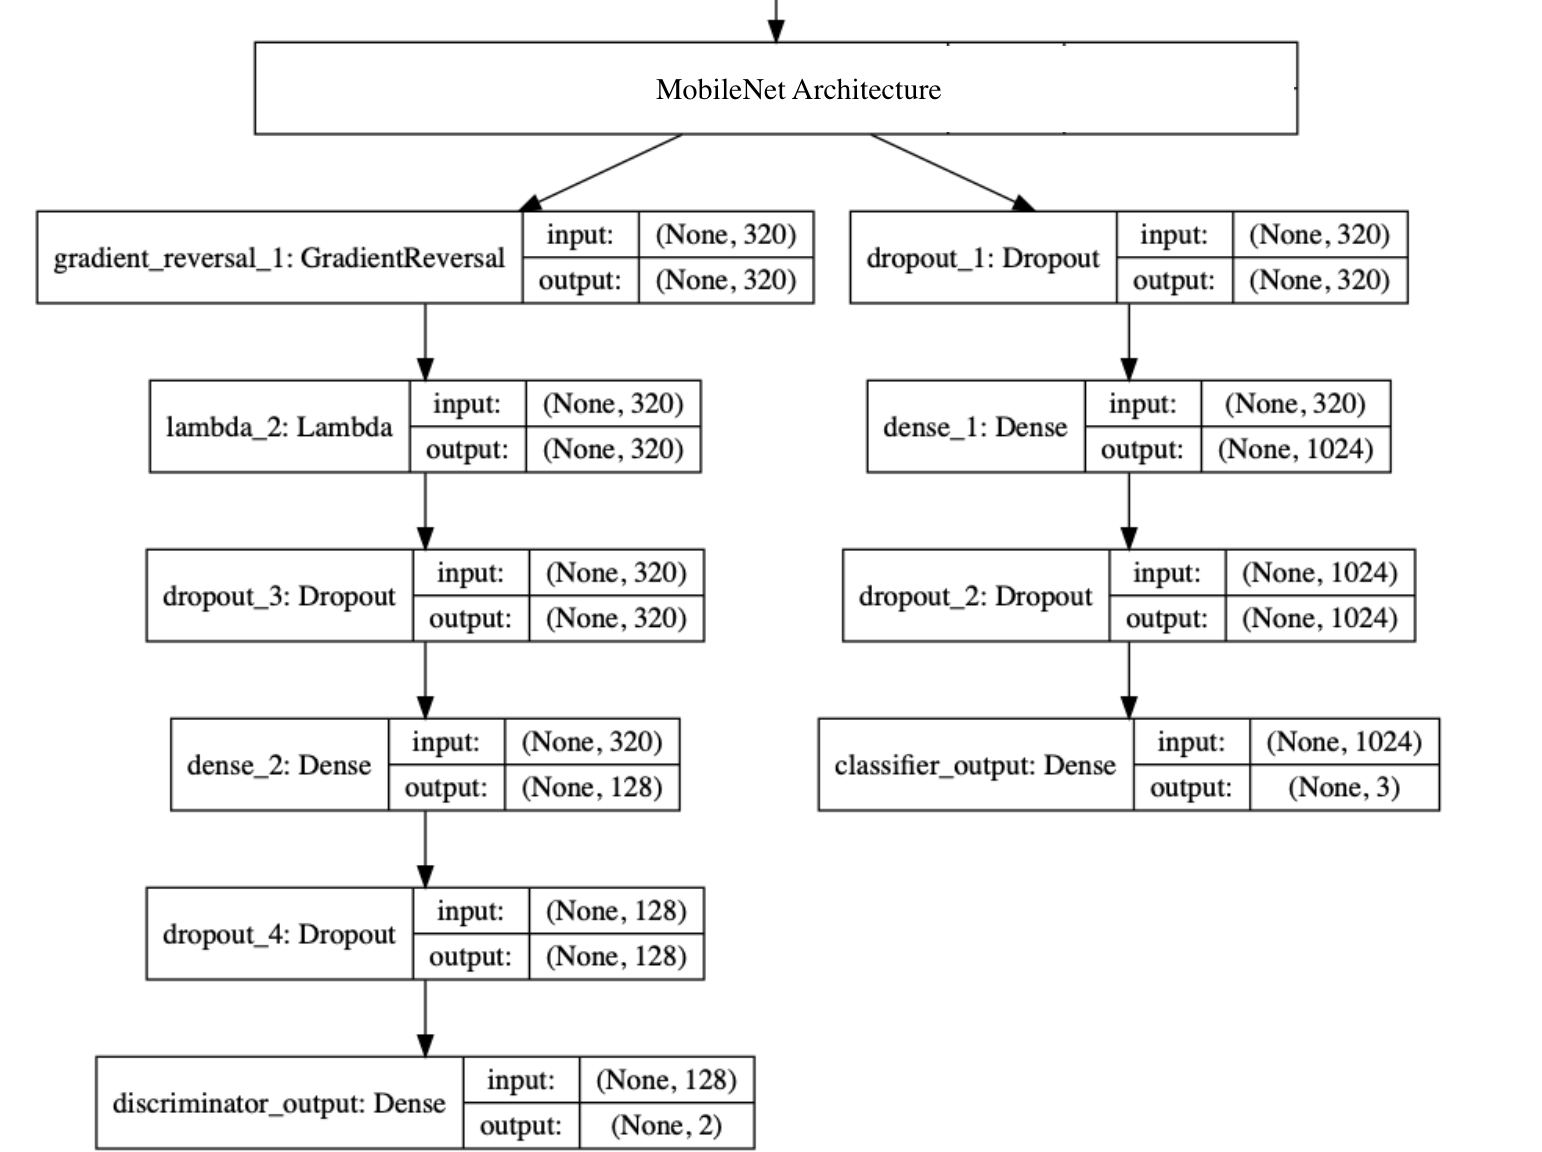
\includegraphics[width=120mm]{Images/Dann_arc.png}
 
 \textbf{Figure 8.} \textit{A diagram showing the added layers to the MobileNet architecture that change the CNN to a DANN CNN, with a gradiant reversal layer for the domain discriminator classifier.}
\end{figure}

If this gradient was zeroed one would be left with a model identical to the classifier discussed previously, based on the MobileNet architecture. If the reversed gradient is not scaled it would have a maximal effect, and would change the weights and biases with an equal effect to the backpropagation from the feature classifier. This would be expected to reduce the effectiveness of the network as the backpropopgation from the domain discriminator would be most destructive in cancelling out the gradients of the feature classifier. In order to assess the effectiveness of a DANN network, a range of linear scaling values, between 0 and 1, were be used to scale the gradient reversal vector.  

